\documentclass[UTF8,11pt]{ctexart}
\usepackage[a4paper,margin=22mm]{geometry}
\usepackage{graphicx,enumitem,amssymb,tabularx}
\usepackage[normalem]{ulem}
\usepackage{xeCJKfntef}
\setlength{\parindent}{0pt}
\setlength{\parskip}{.6em}
\sloppy
\begin{document}
\section*{2020年12月英语四级真题(第1套)}
\subsection*{\textbf{Part I} \textbf{Writing} \textbf{( 30 minutes)}}


\textbf{Directions: }\textbf{\textit{For this part, you are allowed 30 minutes to write on the topic Oulnges in the Way of}} \textbf{\textit{Education. You should write at least 120 words but no more than 180 words.}}


\subsection*{\textbf{Part I} \textbf{Listening Comprehension} \textbf{( 25 minutes)}}


\subsection*{\textbf{Section A}}


. . \textbf{Directions: }\textbf{\textit{In this section, you will hear three news reports. At the end of each news report, you will hear}} \textbf{\textit{two or three questions. Both the news report and the questions will be spoken only once. After you hear a}} \textbf{\textit{question, you must choose the best answer from the four choices marked }}A), B), C) \textbf{\textit{and }}D). \textbf{\textit{Then mark}} \textbf{\textit{the corresponding letter on Answer Sheet 1 with a single line through the centre.}}


\textbf{Questions 1 and 2 are based on the news report you have just heanl.}


\textbf{1.}


\begin{itemize}[leftmargin=2em,itemsep=.2em,topsep=.4em]\item[A.] \textbf{Many people have been attacked by Devil Firefish.}
\item[B.] \textbf{The Mediterranean is a natural habitat of Devil Firefish.}
\item[C.] \textbf{Invasive species are driving away certain native species.}
\item[D.] \textbf{A deadly fish has been spotted in the Mediterranean waters.}
\end{itemize}

\textbf{2.}


\begin{itemize}[leftmargin=2em,itemsep=.2em,topsep=.4em]\item[A.] \textbf{It could badly pollute the surrounding waters.}
\item[B.] \textbf{It could pose a threat to other marine species.}
\item[C.] \textbf{It could disrupt the food chains there.}
\item[D.] \textbf{It could add to greenhouse emissions.}
\end{itemize}

\textbf{Questions 3 and 4 are based on the news report you have just heanl.}


\textbf{3.}


\begin{itemize}[leftmargin=2em,itemsep=.2em,topsep=.4em]\item[A.] \textbf{Cars will not be allowed to enter the city.}
\item[B.] \textbf{Pedestrians will have free access to the city.}
\item[C.] \textbf{About half of its city center will be closed to cars.}
\item[D.] \textbf{Buses will be the only vehicles allowed on its streets.}
\end{itemize}

\textbf{4.}


\begin{itemize}[leftmargin=2em,itemsep=.2em,topsep=.4em]\item[A.] \textbf{The unbearable traffic noise.}
\item[B.] \textbf{The worsening global warming.}
\item[C.] \textbf{The ever-growing cost of petrol.}
\item[D.] \textbf{The rising air pollution in Paris.}
\end{itemize}

\textbf{Questions 5 to 7 are based on the news report you have just heard}


\textbf{5.}


\begin{itemize}[leftmargin=2em,itemsep=.2em,topsep=.4em]\item[A.] \textbf{His house was burnt down in a fire.}
\item[B.] \textbf{Many of his possessions were stolen.}
\item[C.] \textbf{His good luck charm sank into the sea.}
\item[D.] \textbf{His fishing boat got wrecked on a rock.}
\end{itemize}

\textbf{6.}


\begin{itemize}[leftmargin=2em,itemsep=.2em,topsep=.4em]\item[A.] \textbf{Change his fishing locations.}
\item[B.] \textbf{Find a job in a travel agency.}
\item[C.] \textbf{Sell the pearl he had kept for years.}
\item[D.] \textbf{Spend a few nights on a small island.}
\end{itemize}

\textbf{7.}


\begin{itemize}[leftmargin=2em,itemsep=.2em,topsep=.4em]\item[A.] \textbf{His pearl could be displayed in a museum.}
\item[B.] \textbf{His monstrous pearl was extremely valuable.}
\item[C.] \textbf{The largest pearl in the world weighs 14 pounds.}
\item[D.] \textbf{A New York museum has the world's biggest pearl.}
\end{itemize}

\subsection*{\textbf{Section B}}


\textbf{Directions: }\textbf{\textit{In this section, you will hear two long conversations. At the end of each conversation, you will}} \textbf{\textit{hear four questions. Both the conversation and the questions will be spoken only once. After you hear a}} \textbf{\textit{question }}\textbf{, }\textbf{\textit{you must choose the best answer from the four choices marked A) }}\textbf{, }\textbf{\textit{B) }}\textbf{, C) }\textbf{\textit{and }}\textbf{D) . }\textbf{\textit{Then mark}} \textbf{\textit{the corresponding letter on Answer Sheet 1 with a single line through the centre.}}


\textbf{Questions 8 to 11 are based on the conversation you have just heard.}


\textbf{8.}


\begin{itemize}[leftmargin=2em,itemsep=.2em,topsep=.4em]\item[A.] \textbf{It boasts a fairly long history.}
\item[B.] \textbf{It has over 50 business partners.}
\item[C.] \textbf{It has 75 offices around the world.}
\item[D.] \textbf{It produces construction materials.}
\end{itemize}

\textbf{9.}


\begin{itemize}[leftmargin=2em,itemsep=.2em,topsep=.4em]\item[A.] \textbf{It was started by his father.}
\item[B.] \textbf{It has about 50 employees.}
\item[C.] \textbf{It is over 100 years old.}
\item[D.] \textbf{It is a family business.}
\end{itemize}

\textbf{10.}


\begin{itemize}[leftmargin=2em,itemsep=.2em,topsep=.4em]\item[A.] \textbf{Outdated product design.}
\item[B.] \textbf{Loss of competitive edge.}
\item[C.] \textbf{Shortage of raw material supply.}
\item[D.] \textbf{Legal disputes in many countries.}
\end{itemize}

\textbf{11.}


\begin{itemize}[leftmargin=2em,itemsep=.2em,topsep=.4em]\item[A.] \textbf{Introducing innovative marketing strategies.}
\item[B.] \textbf{Seeking new ways .to increase its exports.}
\item[C.] \textbf{Providing training for its staff members.}
\item[D.] \textbf{Conducting a financial analysis for it.}
\end{itemize}

\textbf{Questions 12 to 15 are based on the conversation you have just heard.}


\textbf{12.}


\begin{itemize}[leftmargin=2em,itemsep=.2em,topsep=.4em]\item[A.] \textbf{She is a real expert at house decorations.}
\end{itemize}

\noindent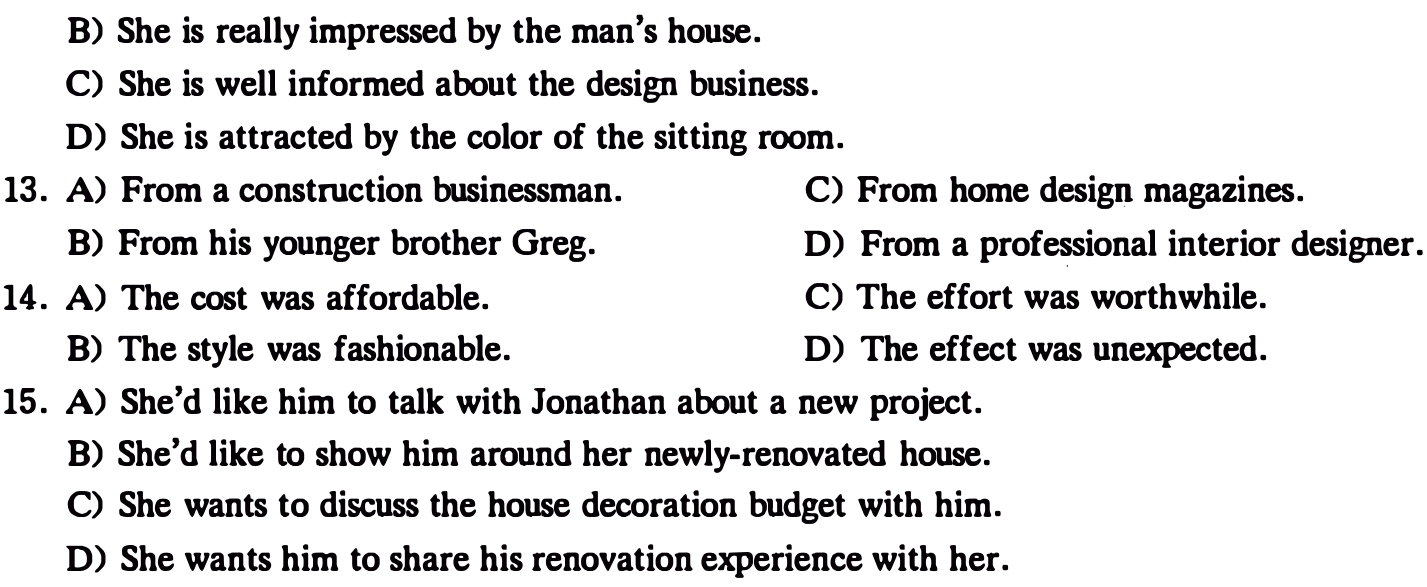
\includegraphics[width=\linewidth,height=.8\textheight,keepaspectratio]{2020-12-01.assets/char-002-line-014.png}\par

\subsection*{\textbf{Section C}}


\textbf{Directions: }\textbf{\textit{In this section, you will hear three passages. At the end of each passage, you will hear three or}} \textbf{\textit{four questions. Both the }}\textbf{passage }\textbf{\textit{and the questions will be spoken only once. After you hear a question }}\textbf{, }\textbf{\textit{you}} \textbf{\textit{must choose the best answer from the four choices marked A }}\textbf{) , }\textbf{\textit{B }}\textbf{) , C ) }\textbf{\textit{and D }}\textbf{) . }\textbf{\textit{Then mark the}} \textbf{\textit{co"esponding letter on Answer Sheet 1 with a single line through the centre.}}


\textbf{Questions 16 to 18 are based on the passage you have just heard.}


\textbf{16.}


\begin{itemize}[leftmargin=2em,itemsep=.2em,topsep=.4em]\item[A.] \textbf{Paying hospital bills for emergency cases.}
\item[B.] \textbf{Doing research on ear, nose and throat diseases.}
\item[C.] \textbf{Removing objects from patients' noses and ears.}
\item[D.] \textbf{Providing routine care for small children.}
\end{itemize}

\textbf{17.}


\begin{itemize}[leftmargin=2em,itemsep=.2em,topsep=.4em]\item[A.] \textbf{Children aged one to four are often more curious than older children.}
\item[B.] \textbf{Five- to nine-year-olds are the most likely to put things in their ears.}
\item[C.] \textbf{Many children like to put foreign objects in their mouths.}
\item[D.] \textbf{Many children like to smell things they find or play with.}
\end{itemize}

\textbf{18.}


\begin{itemize}[leftmargin=2em,itemsep=.2em,topsep=.4em]\item[A.] \textbf{They want to attract attention.}
\item[B.] \textbf{They tend to act out of impulse.}
\item[C.] \textbf{They are unaware of the potential risks.}
\item[D.] \textbf{They are curious about these body parts.}
\end{itemize}

\textbf{Questions 19 to 21 are based on the passage you have just heanl.}


\textbf{19.}


\begin{itemize}[leftmargin=2em,itemsep=.2em,topsep=.4em]\item[A.] \textbf{It gave her a used bicycle.}
\item[B.] \textbf{It paid for her English lessons.}
\item[C.] \textbf{It delivered her daily necessities.}
\item[D.] \textbf{It provided her with physical therapy.}
\end{itemize}

\textbf{20.}


\begin{itemize}[leftmargin=2em,itemsep=.2em,topsep=.4em]\item[A.] \textbf{Expanding bike-riding lessons.}
\item[B.] \textbf{Providing free public transport.}
\item[C.] \textbf{Offering walking tours to visitors.}
\item[D.] \textbf{Asking local people for donations.}
\end{itemize}

\textbf{21.}


\begin{itemize}[leftmargin=2em,itemsep=.2em,topsep=.4em]\item[A.] \textbf{It is a sports club.}
\item[B.] \textbf{It is a language school.}
\item[C.] \textbf{It is a counseling center.}
\item[D.] \textbf{It is a charity organizadon.}
\end{itemize}

\noindent
\includegraphics[width=\linewidth,height=.8\textheight,keepaspectratio]{2020-12-01.assets/char-003-line-009.png}\par

\textbf{22.}


\begin{itemize}[leftmargin=2em,itemsep=.2em,topsep=.4em]\item[A.] \textbf{How animals deal with lack of gravity.}
\item[B.] \textbf{How mice interact in a new environment.}
\item[C.] \textbf{How low gravity affects the human body.}
\item[D.] \textbf{How mice imitate human behavior in space.}
\end{itemize}

\textbf{23.}


\begin{itemize}[leftmargin=2em,itemsep=.2em,topsep=.4em]\item[A.] \textbf{They found the space in the cage too small to stay in.}
\item[B.] \textbf{They found it difficult to figure out where they were.}
\item[C.] \textbf{They were not used to the low-gravity environment.}
\item[D.] \textbf{They were not sensitive to the changed environment.}
\end{itemize}

\textbf{24.}


\begin{itemize}[leftmargin=2em,itemsep=.2em,topsep=.4em]\item[A.] \textbf{They continued to behave as they did in the beginning.}
\item[B.] \textbf{They already felt at home in the new environment.}
\item[C.] \textbf{They had found a lot more activities to engage in.}
\item[D.] \textbf{They tried everything possible to escape from the cage.}
\end{itemize}

\textbf{25.}


\begin{itemize}[leftmargin=2em,itemsep=.2em,topsep=.4em]\item[A.] \textbf{They changed their routines in space.}
\item[B.] \textbf{They began to eat less after some time.}
\item[C.] \textbf{They behaved as if they were on Earth.}
\item[D.] \textbf{They repeated their activities every day.}
\end{itemize}

\subsection*{\textbf{Part }I \textbf{Reading Comprehension} \textbf{( 40 minutes)}}


\subsection*{\textbf{Section A}}


\textbf{Directions: }\textbf{\textit{Jn this section, there is a passage with ten blanks. You are required to select one word for each}} \textbf{\textit{blank from a list of choices given in a word bank following the passage. Read the passage through carefully}} \textbf{\textit{before making your choices. Each choice in the bank is identified by a letter. Please mark the co"esponding}} \textbf{\textit{letter for each item on Answer Sheet 2 with a single line through the centre. You may not use any of the}} \textbf{\textit{words in the bank more than once }}.


\textbf{Trust is fundamental to life. If you can't trust anything, life becomes intolerable. You can't have} \textbf{relationships without trust, let alone good ones.}


\textbf{In the workplace, too, trust is} \textbf{\uline{26}} \textbf{. An organization without trust will be full of fear and}


\textbf{\uline{27}} \textbf{. If you work for a boss who doesn't trust their employees to do things right, you'll have a}


\textbf{-28-time. They'll be checking up on you all the time, correcting "mistakes" and-29-reminding you to do this or that. Colleagues who don't trust one another will need to spend more time}


\textbf{\uline{30}} \textbf{their backs than doing any useful work.}


\textbf{Organizations are always trying to cut costs. Think of all the additional tasks caused by lack of trust.} \textbf{\textit{Audit }}\textbf{('fit) departments only exist because of it. Companies keep large volumes of-31- because} \textbf{they don't trust their suppliers, their contractors or their customers. Probably more than half of all}


\textbf{administrative work is only there because of an ever-existing sense that "you can't trust anyone these} \textbf{days. " If even a small part of such valueless work could be} \textbf{\uline{32}} \textbf{, the savings would run into millions} \textbf{of dollars.}


\noindent
\includegraphics[width=\linewidth,height=.8\textheight,keepaspectratio]{2020-12-01.assets/char-004-line-001.png}\par

\begin{itemize}[leftmargin=2em,itemsep=.2em,topsep=.4em]\item[A.] \textbf{constantly}
\item[B.] \textbf{credible}
\item[C.] \textbf{essential}
\item[D.] \textbf{exploring}
\item[E.] \textbf{gather}
\item[F.] \textbf{load}
\item[G.] \textbf{miserable}
\item[H.] \textbf{pressure}
\item[I.] \textbf{properly}
\item[J.] \textbf{records} \textbf{0) watching}
\item[K.] \textbf{removed}
\item[L.] \textbf{stacks}
\item[M.] \textbf{suspicion}
\item[N.] \textbf{tracked}
\end{itemize}

\subsection*{\textbf{Section B}}


\noindent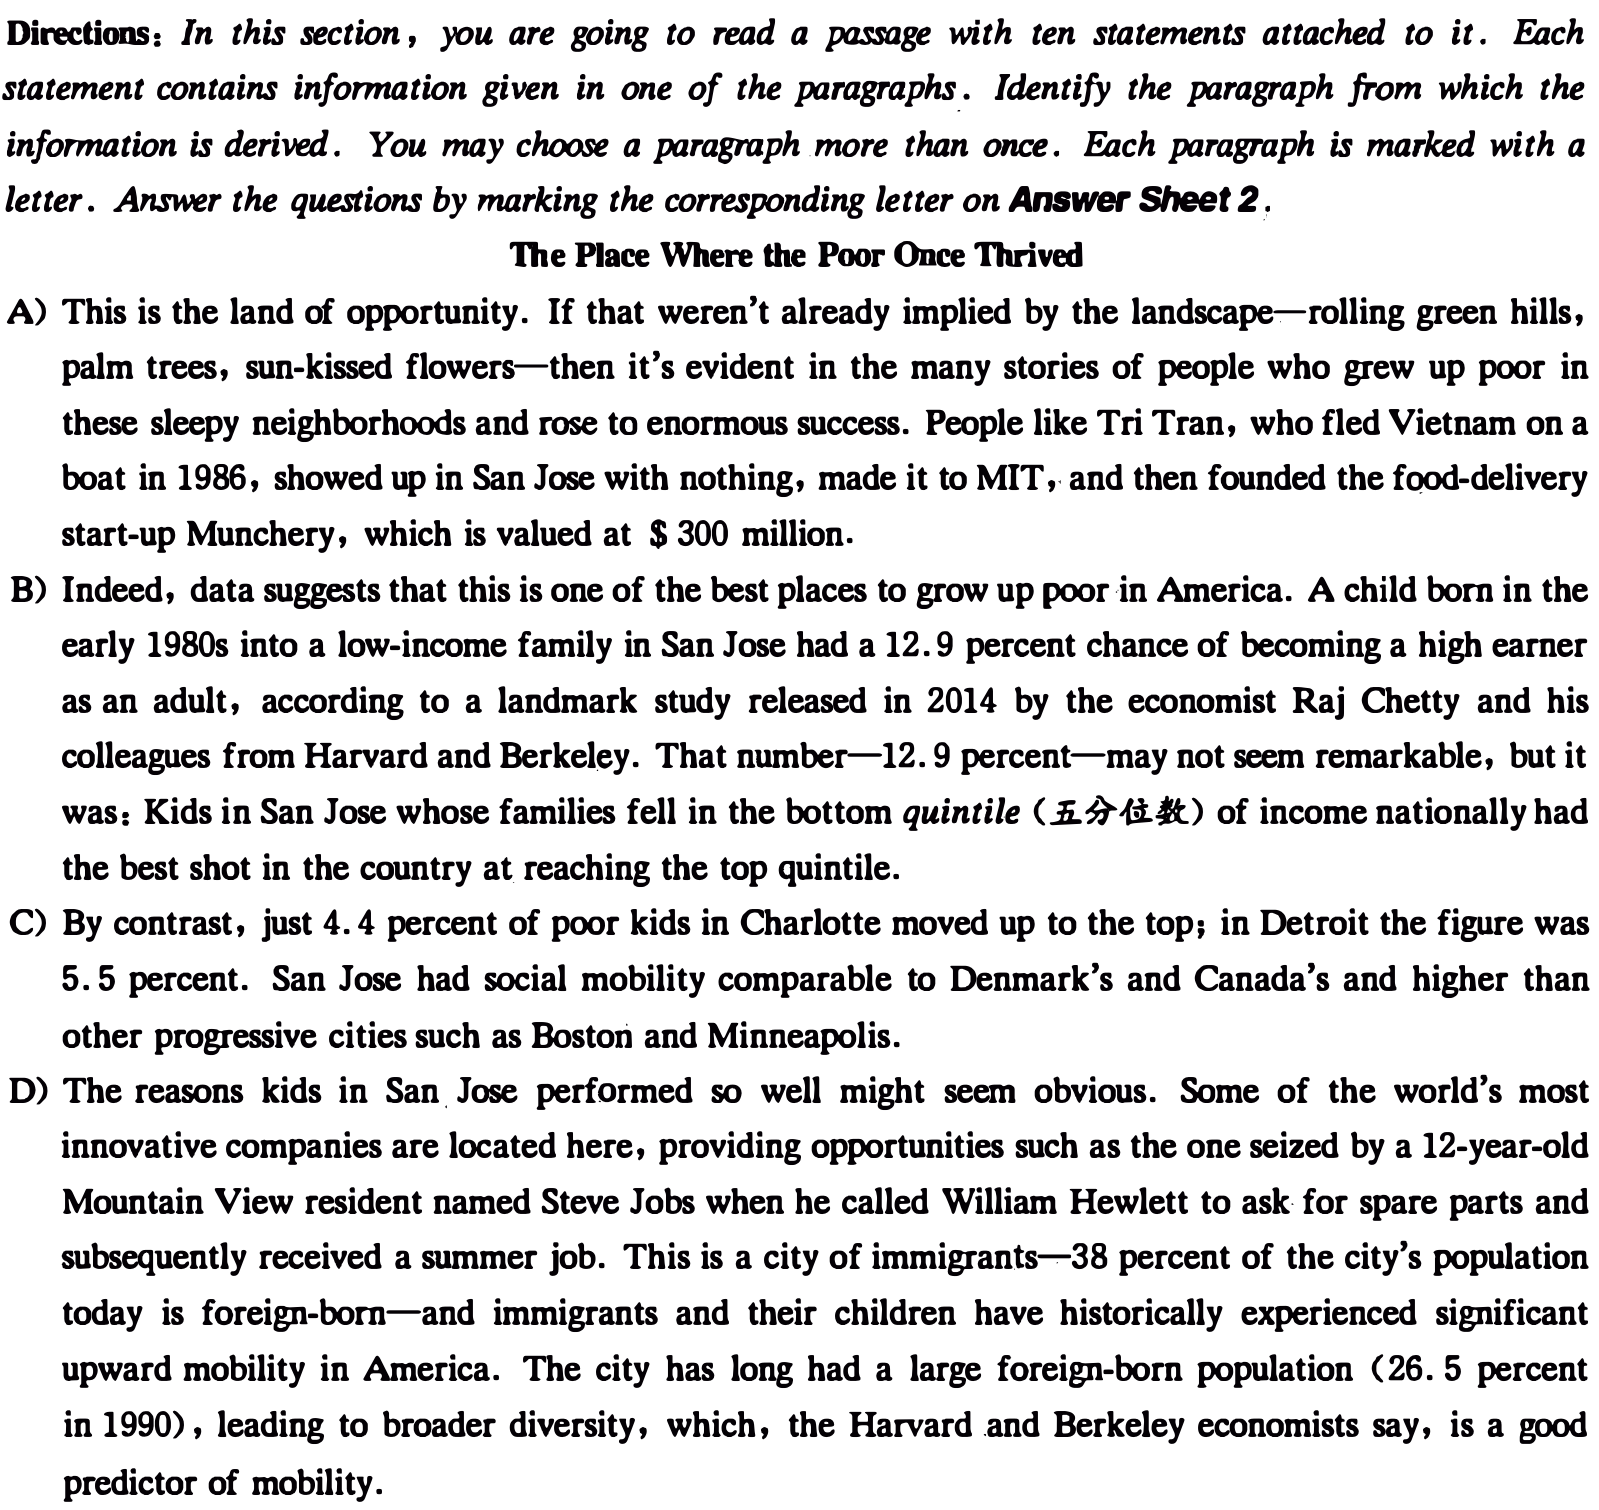
\includegraphics[width=\linewidth,height=.8\textheight,keepaspectratio]{2020-12-01.assets/char-004-line-004.png}\par

\noindent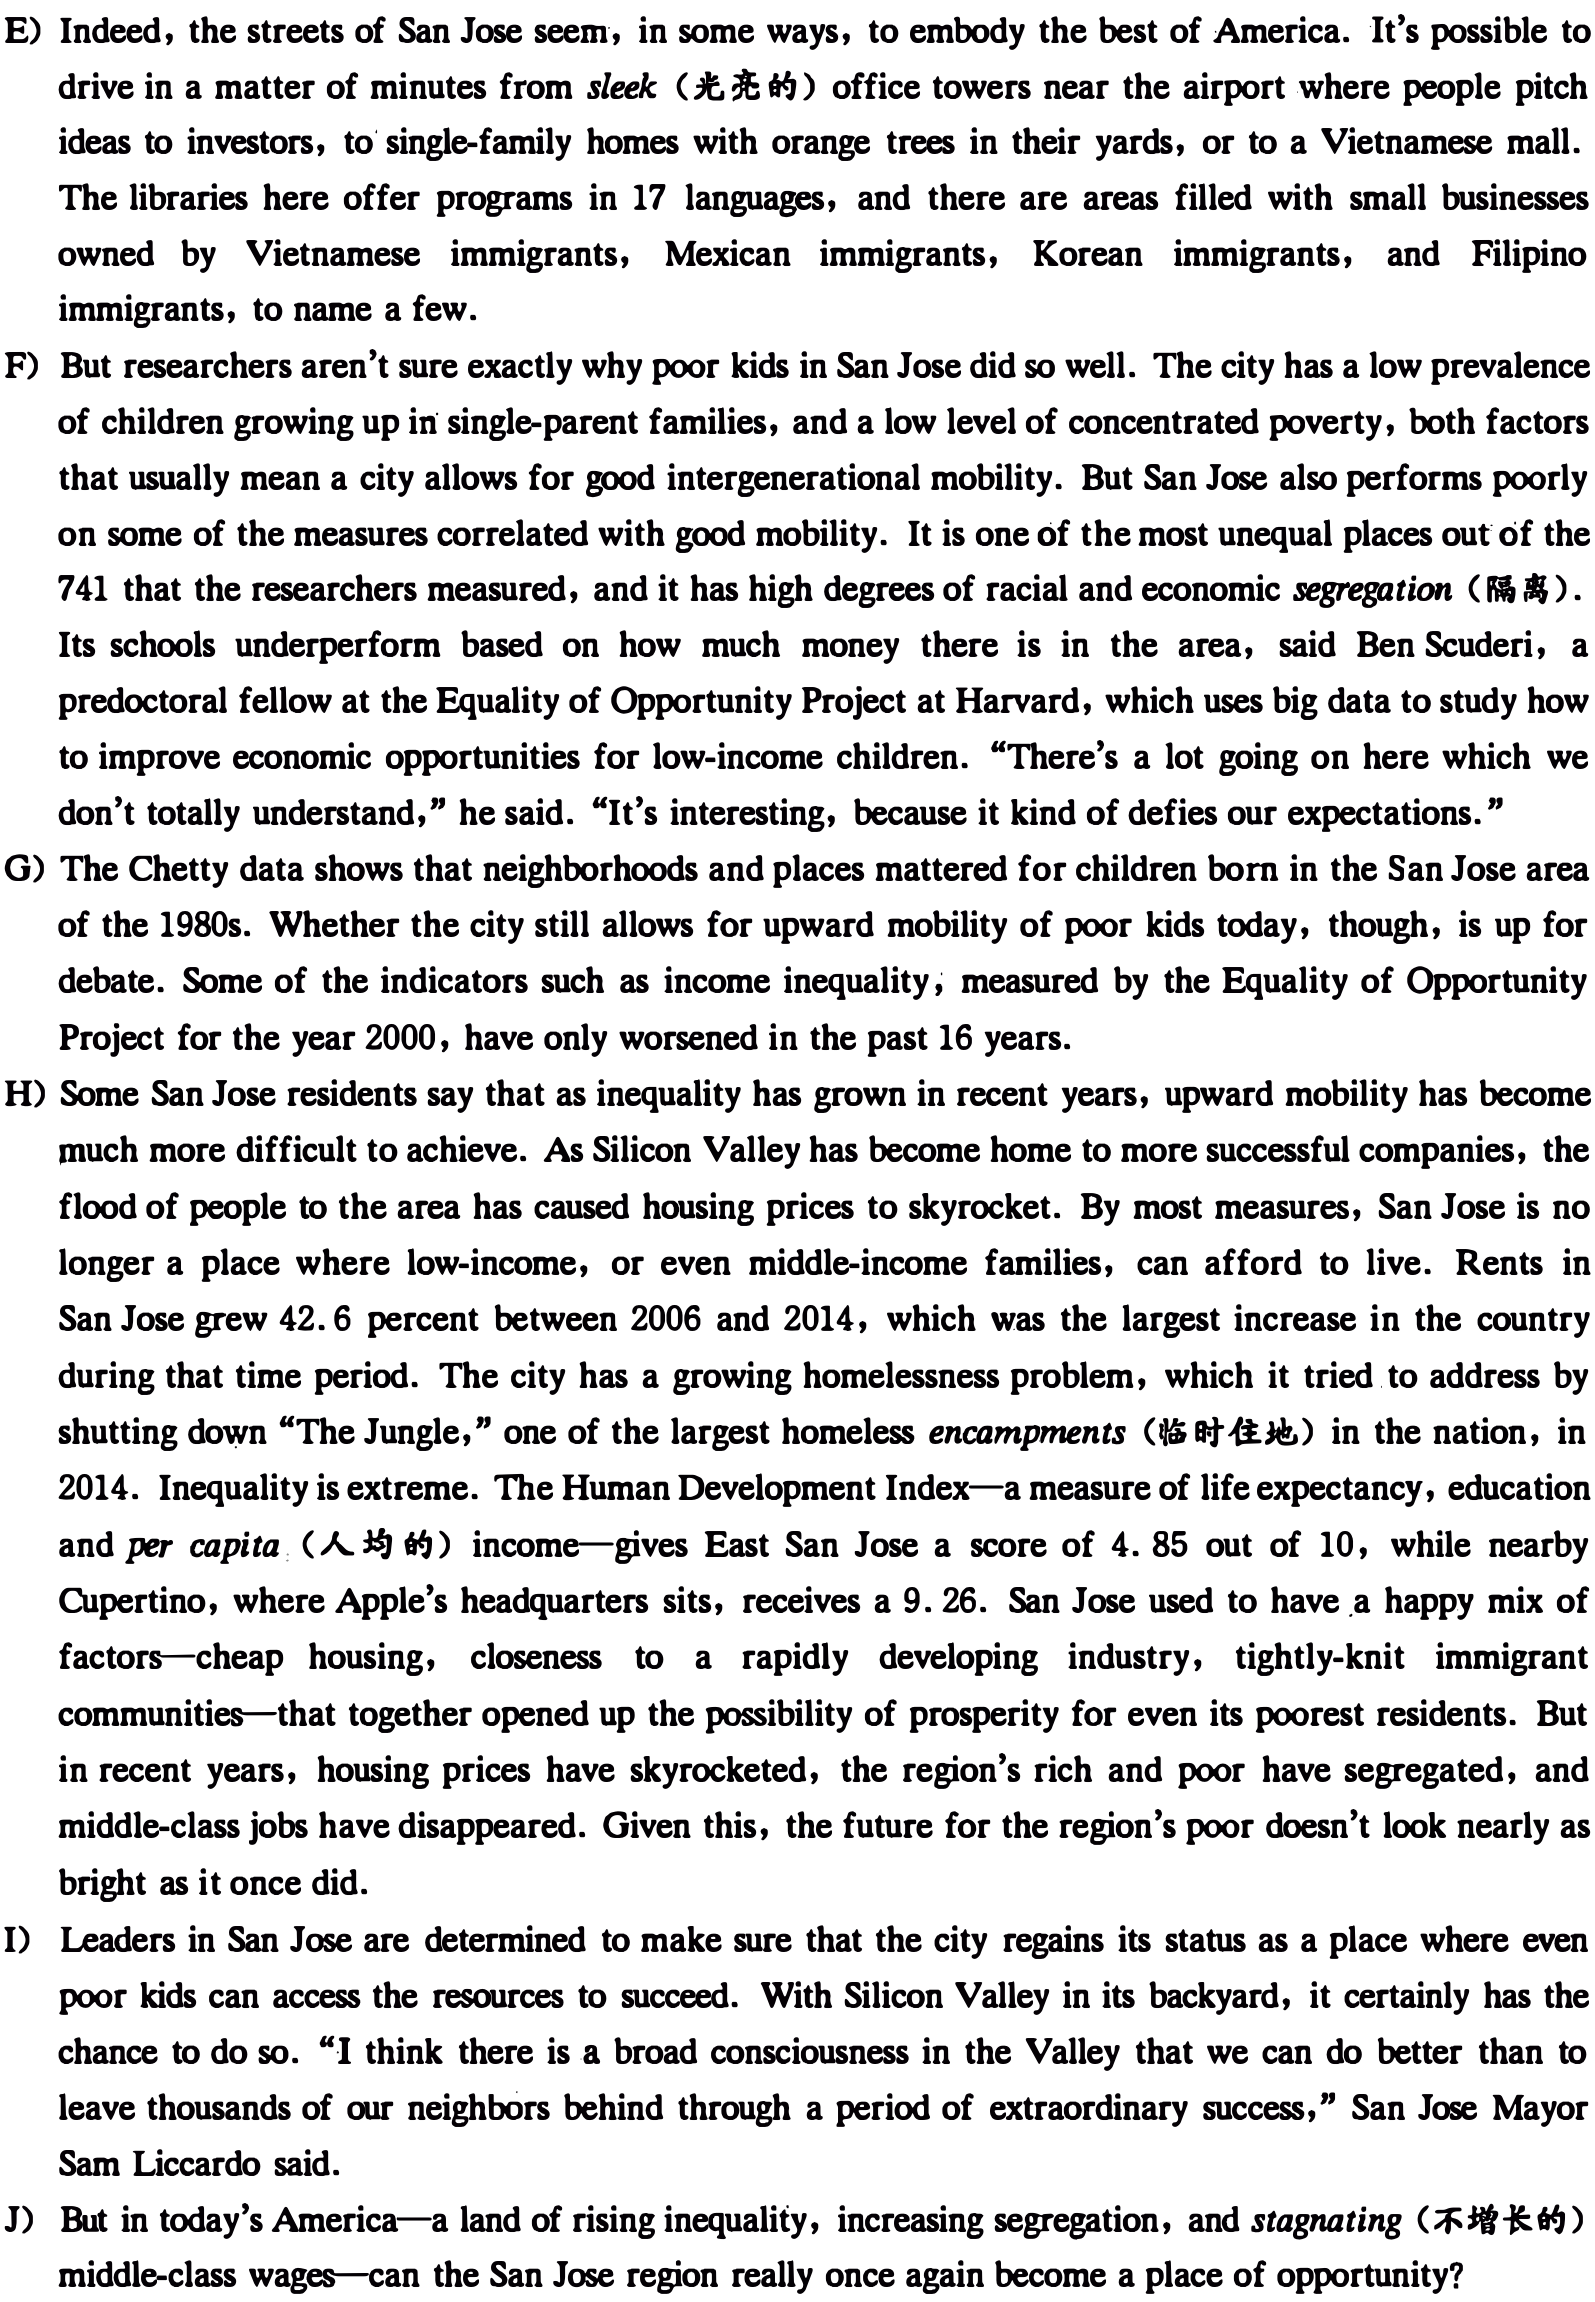
\includegraphics[width=\linewidth,height=.8\textheight,keepaspectratio]{2020-12-01.assets/char-005-line-000.png}\par

K) \textbf{The idea that those at the bottom can rise to the top is central to America's ideas about itself. That} \textbf{such mobility has become more difficult in San Jose raises questions about, the endurance of that} \textbf{foundational belief. After all, if the one-time land of opportunity can't be fixed, what does that say} \textbf{for the rest of America?}


\textbf{36. According to some people living in San Jose, it has become much harder for the poor to get ahead due}


\textbf{to the increased inequality.}


\textbf{37. In American history, immigrants used to have a good chance to move upward in society.}


\textbf{38. If the problems of San Jose can't be solved, one of America's fundamental beliefs about itself can be}


\textbf{shaken.}


\textbf{39. San Jose was among the best cities in America for poor kids to move up the social ladder ..}


\noindent
\includegraphics[width=\linewidth,height=.8\textheight,keepaspectratio]{2020-12-01.assets/char-006-line-007.png}\par

\textbf{41. San Jose's officials are resolved to give poor kids access to the resources necessary for success in life.}


\textbf{42. San Jose appears to manifest some of the best features of America.}


\textbf{43. As far as social mobility is concerned, San Jose beat many other progressive cities in America.}


\textbf{44. Due to some changes like increase,s in housing prices in San Jose, the prospects for its poor people have}


\textbf{dimmed.}


\textbf{45. Researchers do not have a clear idea why poor children in San Jose achieved such great success several}


\textbf{decades ago.}


\subsection*{\textbf{Section C}}


\noindent
\includegraphics[width=\linewidth,height=.8\textheight,keepaspectratio]{2020-12-01.assets/char-006-line-016.png}\par

\subsection*{\textbf{Passage One}}


\textbf{Questions 46 to SO are based on the following pamage.}


\textbf{Three children in every classroom have a diagnosable mental health condition. Half of these are} \textbf{behavioural disorders, while one third are emotional disorders such as stress, anxiety and depression,} \textbf{which often become outwardly apparent through self-harm. There was an astonishing 52 per cent jump in} \textbf{hospital admissions for children and young people who had harmed themselves between 2009 and 2015.}


\textbf{Schools and teachers have consistently reported the scale of the problem since 2009. Last year, over} \textbf{half of teachers reported that more of. their pupils experience mental health problems than in the past. But} \textbf{teachers also consistently report how ill-equipped they feel to meet pupils' mental health needs, and often}


\noindent
\includegraphics[width=\linewidth,height=.8\textheight,keepaspectratio]{2020-12-01.assets/char-006-line-021.png}\par

\subsection*{\textbf{Part of the reason for the increased pressure on . schools is that there are now fewer ' early}}


\textbf{\textit{intervention }}\textbf{( -ril)' and low-level mental health services based in the community. Cuts to local authority} \textbf{\textperiodcentered{}budgets since 2010 have resulted in a significant decline of these services, despite strong evidence of their} \textbf{effectiveness in preventing crises further down the line.}


\textbf{The only way to break the pressures on both mental health services and schools is to reinvest in early} \textbf{intervention services inside schools.}


\noindent
\includegraphics[width=\linewidth,height=.8\textheight,keepaspectratio]{2020-12-01.assets/char-006-line-025.png}\par

\textbf{see young people more than any other service, which gives them a unique ability to get to hard-to-reach} \textbf{children and young people and build meaningful relationships with them over time. Recent studies have} \textbf{shown that children and young people\_largely prefer to see a counsellor in school rather than in an.outside} \textbf{environment. :Young people have reported that for low-level conditions such as stress and anxiety, a} \textbf{clinical setting can sometimes be }\textbf{\textit{daunting }}\textbf{(}\(\blacklozenge\)\textbf{A. -,!p }\textit{ffe }\textbf{\{rlJ) .} \textbf{There are already, examples of innovative schools which combine mental health and well being} \textbf{provision with a strong academic curriculum. This• will, though, require a huge cultural shift. Politicians,} \textbf{policymakers, commissioners and school leaders must be brave enough to make the leap towards} \textbf{reimagining schools as providers of health as well as education services.}


\textbf{46. What are teachers complaining about?}


\begin{itemize}[leftmargin=2em,itemsep=.2em,topsep=.4em]\item[A.] \textbf{There are too many students requiring special attention.}
\item[B.] \textbf{They are under too much stress counselling \textperiodcentered{}needy students.}
\item[C.] \textbf{Schools are inadequately equipped to implement any intervention.}
\item[D.] \textbf{They lack the necessary resources to address pupils' mental problems.}
\end{itemize}

\textbf{47. What do we learn from the passage about community health services in Britain?}


\begin{itemize}[leftmargin=2em,itemsep=.2em,topsep=.4em]\item[A.] \textbf{They have deteriorated due to budget cuts.,\textperiodcentered{}}
\item[B.] \textbf{They facilitate local residents' everyday lives.}
\item[C.] \textbf{They prove ineffective in helping mental patients. •}
\item[D.] \textbf{They cover preventative care for the local residents.}
\end{itemize}

\textbf{48. Where does the author suggest mental health services be placed?}


\begin{itemize}[leftmargin=2em,itemsep=.2em,topsep=.4em]\item[A.] \textbf{At home.}
\item[B.] \textbf{At school.}
\item[C.] \textbf{In hospitals.}
\item[D.] \textbf{In communities.}
\end{itemize}

\textbf{49. What do we learn from the recent studies?,}


\begin{itemize}[leftmargin=2em,itemsep=.2em,topsep=.4em]\item[A.] \textbf{Students pref er to rely on peers to relieve stress and anxiety.}
\item[B.] \textbf{Young people are keen on building meaningful relationships.}
\item[C.] \textbf{Students are more comfortable seeking counselling in school.}
\item[D.] \textbf{Young people benefit from various kinds of outdoor activities.}
\end{itemize}

\textbf{50. What does the author mean by a cultural shift (Line 2, Para. 6)?}


\begin{itemize}[leftmargin=2em,itemsep=.2em,topsep=.4em]\item[A.] \textbf{Simplification of schools' academic curriculums.}
\item[B.] \textbf{Parents' involvement in schools' policy-making.}
\item[C.] \textbf{A change in teachers' attitudes to mental health.}
\item[D.] \textbf{A change in the conception of what schools are.}
\end{itemize}

\subsection*{\textbf{Passage Two}}


\textbf{Questions 51 to 55 are based on the following p;mage. •}


\subsection*{\textbf{Picture this: You're at a movie theater food stand loading up on snacks. You have a choice of }a \textbf{small,}}


\textbf{medium or large soda. The small is \$ 3. 50 and the large is \$ 5. 50. It's a tough decision: The small size} \textbf{may not last you through the whole movie, but \$ 5. 50 for some sugary drink seems ridiculous. But there's} \textbf{a third option, a medium soda for \$ 5. 25. Medium may be the perfect amount of soda for you, but the} \textbf{large is only a quarter more. If you're like most people, you end up buying the large ( and -taking a} \textbf{bathroom break midshow).} \textbf{If you're wondering who would buy the medium soda, the answer is almost-no one. In fact, there's a} \textbf{good chance the marketing department purposely priced the medium soda as a }\textbf{\textit{decoy }}\textbf{( it--tif.) , making you} \textbf{more likely to buy the large soda rather than the small.} \textbf{I have written about this peculiarity in human nature before with my friend Dan Ariely, who studied this} \textbf{phenomenon extensively after noticing pricing for }\textbf{\textit{subscriptions }}\textbf{( f.T fl1J) to }\textbf{\textit{The \&onomist. }}\textbf{The digital}


\textbf{subscription was \$ 59, the print subscription was \$ 125, and the print plus\textperiodcentered{} digital subscription was also} \textbf{\$125. No one in their right mind would buy the print subscription when you could get digital as well for} \textbf{the same price, so why was it even an option? Ariely ran an experiment and found that when only the two} \textbf{"real" choices were offered, more people chose the less-expensive digital subscription. But the addition of} \textbf{the bad option made people much more likely to choose the more expensive print plus digital option.} \textbf{Brain scientists call this effect"asymmetric dominance" and it means that people gravitate toward the} \textbf{choice nearest a clearly inferior option. Marketing professors call it the decoy effect, which is certainly} \textbf{easier to remember. Lucky for consumers, almost no one in the business community understands it.} \textbf{The decoy effect works because of the way our brains. assign value when making choices. Value is} \textbf{almost never absolute; rather, we decide an object's value relative to our other choices. If more options} \textbf{are introduced, the value equation changes.}


\textbf{51. Why does the author ask us to imagine buying food in the movie theater?}


\begin{itemize}[leftmargin=2em,itemsep=.2em,topsep=.4em]\item[A.] \textbf{To illustrate people's peculiar shopping behavior.}
\item[B.] \textbf{To illustrate the increasing variety of snacks there.}
\item[C.] \textbf{To show how hard it can be to choose a drink there.}
\item[D.] \textbf{To show how popular snacks are among movie fans.}
\end{itemize}

\textbf{52. Why is the medium soda priced the way it is?}


\begin{itemize}[leftmargin=2em,itemsep=.2em,topsep=.4em]\item[A.] \textbf{To attract more customers to buy it.}
\item[B.] \textbf{To show the price matches the amount.}
\item[C.] \textbf{To ensure customers drink the right amount of soda.}
\item[D.] \textbf{To make customers believe they are getting a bargain.}
\end{itemize}

\textbf{53. What do we learn from Dan Ariely's experiment?}


\begin{itemize}[leftmargin=2em,itemsep=.2em,topsep=.4em]\item[A.] \textbf{Lower-priced goods attract more customers.}
\item[B.] \textbf{\textit{The}}
\item[C.] \textbf{\textit{The Economist's }}\textbf{print edition turns out to sell the best.}
\item[D.] \textbf{More readers choose the digital over the print edition.}
\item[F.] \textbf{\textit{conomist }}\textbf{'s promotional strategy works.}
\end{itemize}

\textbf{54. For what purpose is "the bad option" (Line 7, Para. 3) added? .}


\begin{itemize}[leftmargin=2em,itemsep=.2em,topsep=.4em]\item[A.] \textbf{To cater to the peculiar needs of some customers.}
\item[B.] \textbf{To help customers to make more rational choices.}
\item[C.] \textbf{To\textperiodcentered{} trap customers into buying the more pricey item.}
\item[D.] \textbf{To provide customers with a greater variety of goods.}
\end{itemize}

\textbf{55. How do we assess the value of a commodity, according to the passage?}


\begin{itemize}[leftmargin=2em,itemsep=.2em,topsep=.4em]\item[A.] \textbf{By considering its usefulness.}
\item[B.] \textbf{By comparing it with other choices.}
\item[C.] \textbf{By taking its quality into account.}
\item[D.] \textbf{By examining its value equation.}
\end{itemize}

\subsection*{Part \textit{N} \textbf{Translation} \textbf{(30 minutes)}}


\subsection*{\textbf{Directions: }\textbf{\textit{For this part }}, \textbf{\textit{you are allowed 30 minutes to translate a passage from Chinese into English. You}}}


\subsection*{\textbf{\textit{should write your answer on Answer Sheet 2 .}}}


\noindent
\includegraphics[width=\linewidth,height=.8\textheight,keepaspectratio]{2020-12-01.assets/char-008-line-014.png}\par
\end{document}